% \xsection{myblue}{nJets}

\begin{frame}{Building number of jets label}%\todo[inline]{Fabricio}
    \textit{Not currently in use, but we investigate if it could help.} \\
    Trained a BDT for labeling events by the number of jets using the $y$ and $m$ variables.
    \begin{itemize}
        \item We use 20 input variables:
        \begin{itemize}
            \item The masses of individual and combined (up to 4) jets, $m$.
            \item The $y_{ij}$ values from the jet clustering algorithm.
        \end{itemize}
        \item The target used for training is the true number of hadronic jets.
        \item Trained the BDT using 100k events from the signal sample.
        \item Performed a randomized search on the following hyper parameters (\textbf{best}):
        \begin{itemize}
            \item \texttt{eta}: \quad\quad\quad\quad\quad\quad\quad [0.05, 0.10, \textbf{0.20}, 0.30, 0.35] ,
            \item \texttt{max\_depth}: \quad\quad\quad\quad [2, 3, 4, \textbf{5}, 6],
            \item \texttt{gamma}: \quad\quad\quad\quad\quad\quad [3, 1, \textbf{0.5}, 1e-01, 1e-02],
            \item \texttt{colsample\_bytree}: \hspace{0.3em} [0.5, \textbf{0.6}, 0.7].
        \end{itemize}
        % \item H$\to$ cc performance?
    \end{itemize}
\end{frame}

\begin{frame}{Building number of jets label}

     \begin{columns}[c,onlytextwidth]
      \begin{column}{0.60\textwidth}
        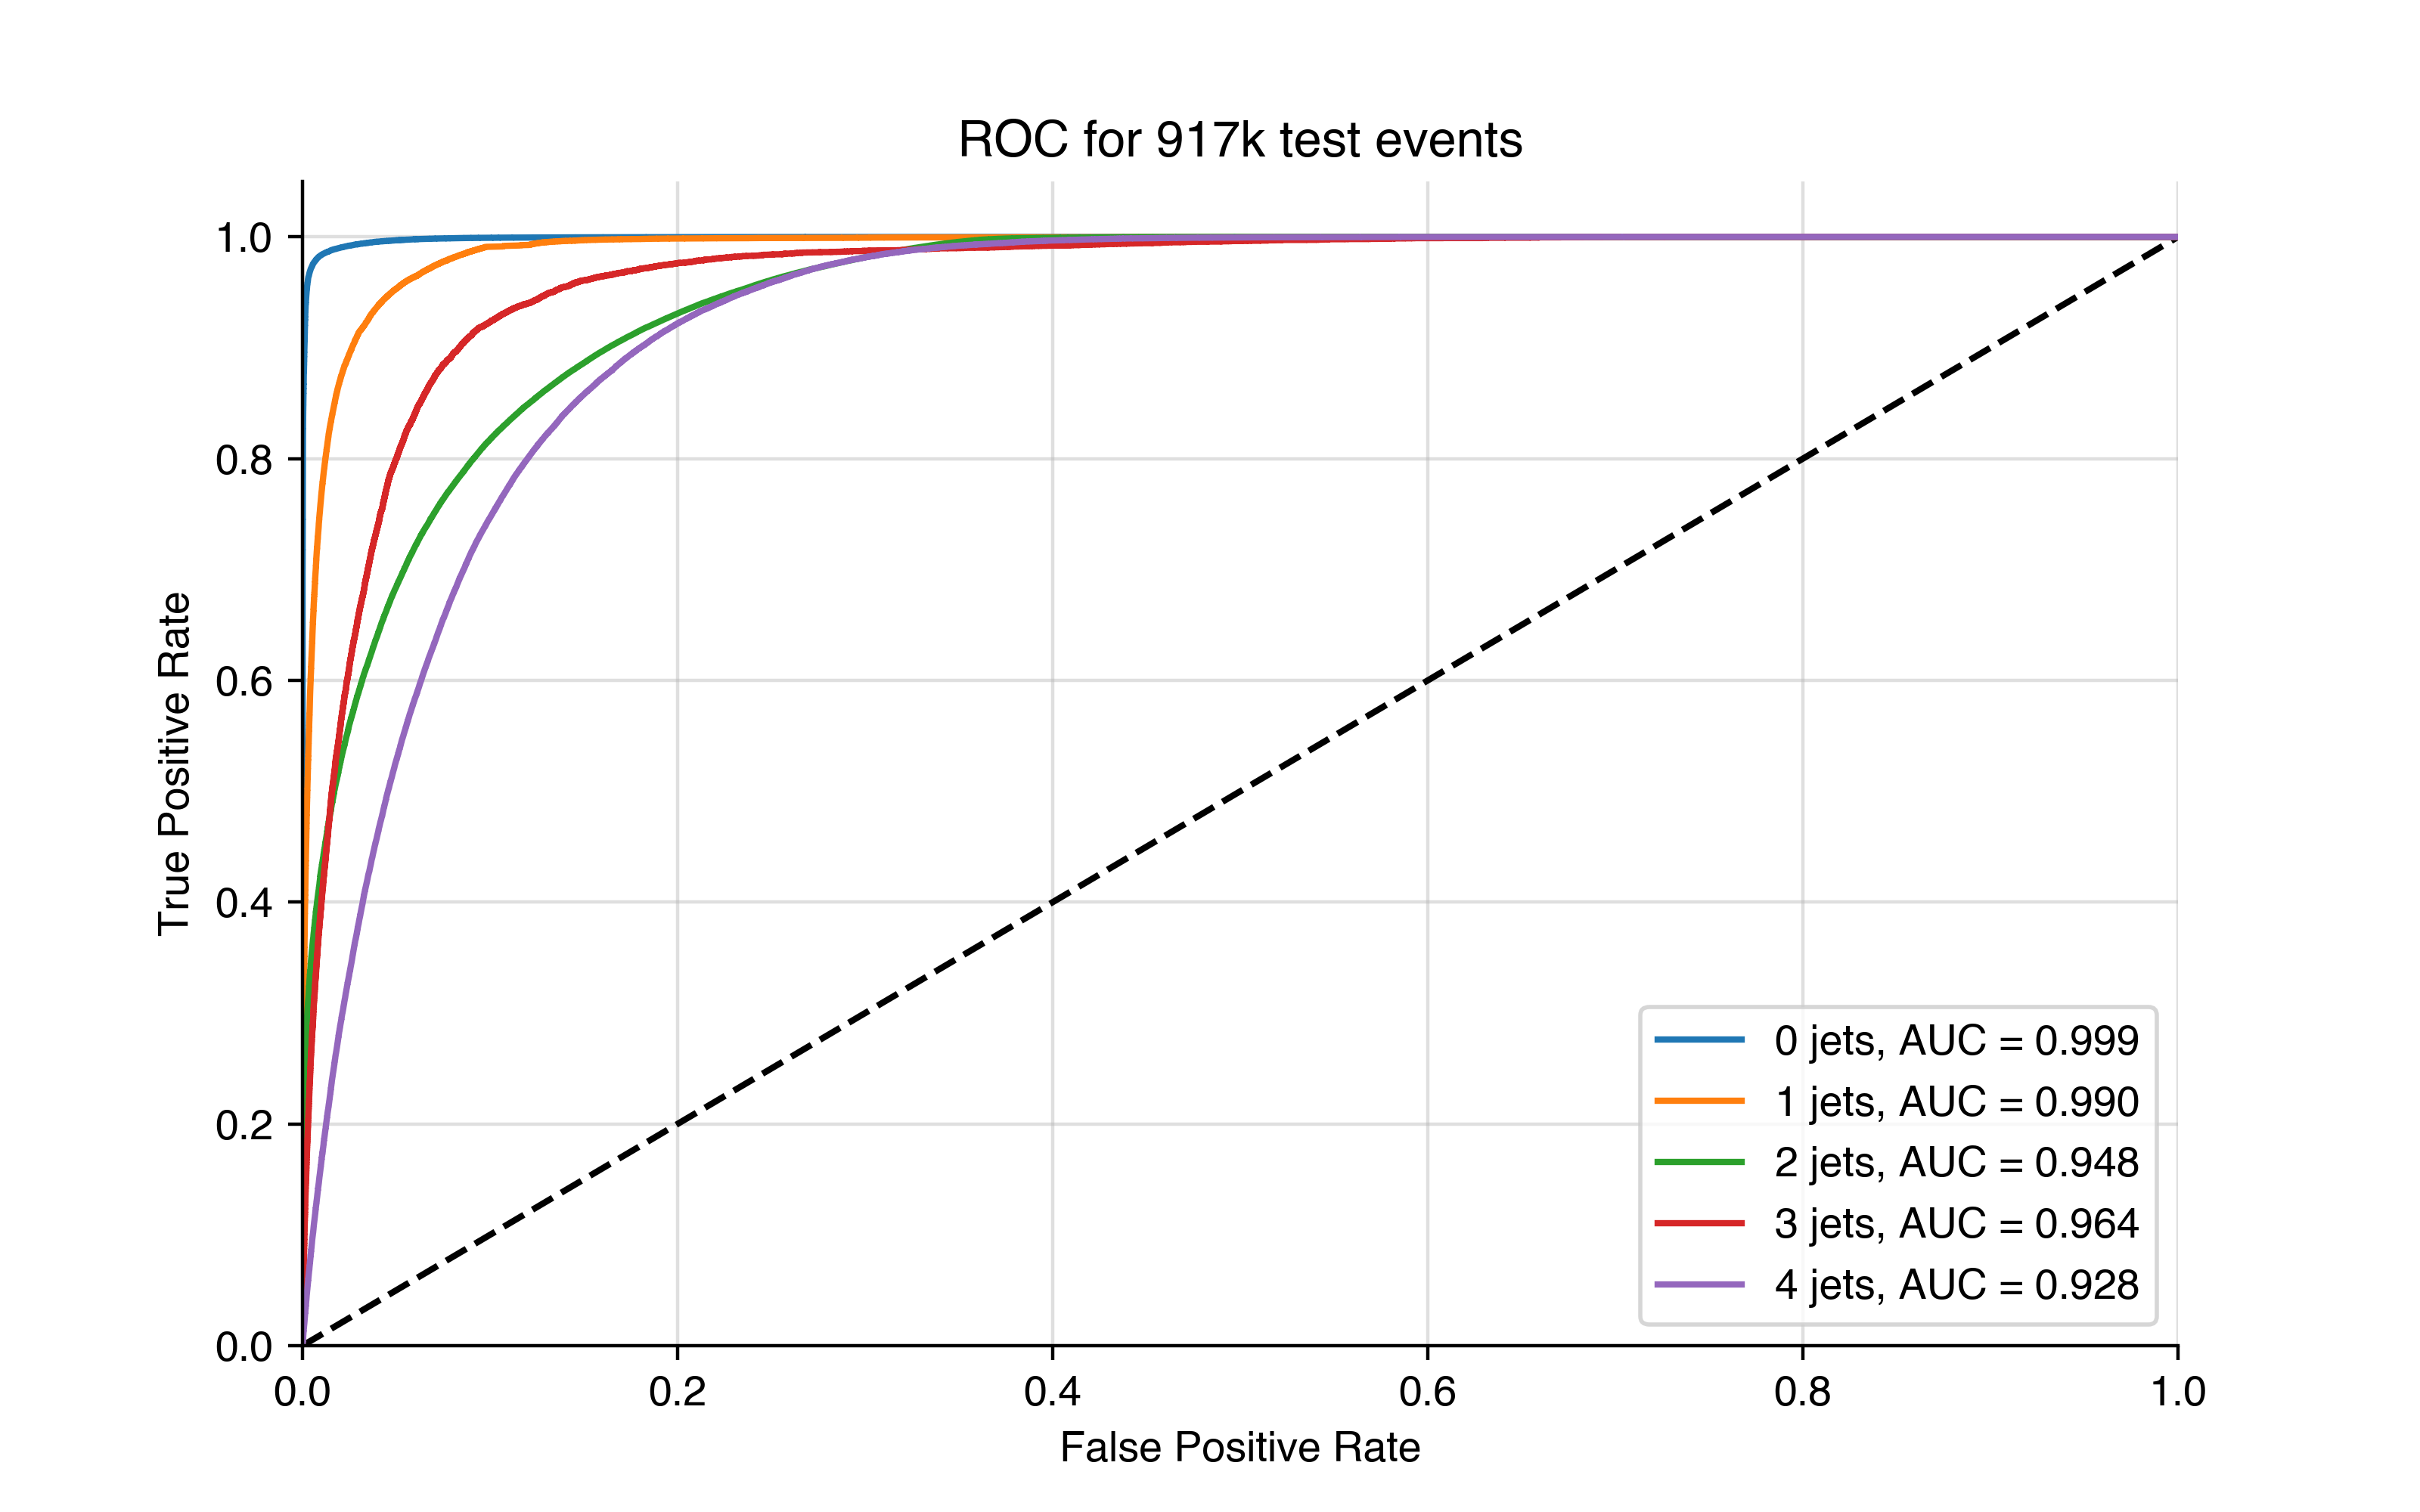
\includegraphics[width=0.95\textwidth]{fabricio/simple_event_vector__100k_roc.png}
      \end{column}
      \begin{column}{0.40\textwidth}
        \begin{itemize}
            \item Multiclass ROC using one-versus-rest strategy.
            \item Studies in progress to understand how well this classifier performs, particularly when tested in subsets of data (i.e. categories).
            \item Having a \# jets predicted can help us build optimal categories for Higgs BR measurements.
            % \item Comment on H cc performance
            % \item (Discuss) Include n-isolated leptons on target?
        \end{itemize}
      \end{column}
  \end{columns}

\end{frame}